\documentclass[11pt]{article}

\usepackage{lipsum}
\usepackage{amsmath}
\usepackage{amsthm}
\usepackage{amssymb}
\usepackage[utf8]{inputenc}
\usepackage[english]{babel}
\usepackage{graphicx}
\graphicspath{ {images/} }
\usepackage{cite}
\usepackage{caption}
\usepackage{algorithm}
\usepackage{algcompatible}
\usepackage{algpseudocode}

\topmargin 0.0cm
\oddsidemargin 0.2cm
\textwidth 16cm 
\textheight 21cm
\footskip 1.0cm

\newenvironment{sciabstract}{%
\begin{quote} \bf}
{\end{quote}}

\renewcommand\refname{References and Notes}

% The following lines set up an environment for the last note in the
% reference list, which commonly includes acknowledgments of funding,
% help, etc.  It's intended for users of BibTeX or the {thebibliography}
% environment.  Users who are hand-coding their references at the end
% using a list environment such as {enumerate} can simply add another
% item at the end, and it will be numbered automatically.

\newcounter{lastnote}
\newenvironment{scilastnote}{%
\setcounter{lastnote}{\value{enumiv}}%
\addtocounter{lastnote}{+1}%
\begin{list}%
{\arabic{lastnote}.}
{\setlength{\leftmargin}{.22in}}
{\setlength{\labelsep}{.5em}}}
{\end{list}}

\title{Nearest Neighbor Search in Hilbert Space} 


% Place the author information here.  Please hand-code the contact
% information and notecalls; do *not* use \footnote commands.  Let the
% author contact information appear immediately below the author names
% as shown.  We would also prefer that you don't change the type-size
% settings shown here.

\author
{Neel V. Rakholia,$^{1\ast}$ William B. March,$^{2}$ George Biros$^{2}$\\
\\
\normalsize{$^{1}$Department of Applied Mathematics and Applied Physics,}\\
\normalsize{Columbia University,}
\normalsize{New York, NY 10027, USA}\\
\normalsize{$^{2}$Institute for Computational Engineering and Science,}\\
\normalsize{University of Texas at Austin,}
\normalsize{Austin, TX 78705, USA}\\
\\
\normalsize{$^\ast$To whom correspondence should be addressed; E-mail:  nvr2105@columbia.edu}
}

% Include the date command, but leave its argument blank.
\date{}

\begin{document}

% Double-space the manuscript.
%\baselineskip24pt
% Make the title.
\maketitle 

\paragraph{Abstract.} Significant work has been done on addressing the problem of nearest neighbor (NN) search in Euclidean Space. Notable is the wealth of literature on search techniques involving the use of trees. Kd-trees and Ball trees are among the more commonly used data structures to speed up NN search. Surprisingly little work however has been done on using trees to find nearest neighbors in general metric spaces.
\\
\indent In this paper we undertake a study of vantage point trees (VP-trees), and analyze their effectiveness in finding NN for kernel based distance metrics. We also propose a new algorithm for searching VP-trees: an approximate random tree search algorithm. Previous work on VP-trees has focused on a priority queue based search, which is not very effective for even moderately high dimensional data. Our approach is unique in this regard.
\\
\indent For an RBF-kernel based distance metric, 4,500,000 training points and 18 features, NN search on 500,000 query points using the random trees search method yielded 90 percent accuracy with only about 1 percent of total distance evaluations, an improvement of about 2 orders of magnitude. 

\paragraph{Keywords.} Nearest Neighbor Algorithms, Tree Codes, Metric Spaces, Data Analysis, VP-Trees, Machine Learning

\section{Introduction} 
\paragraph{Nearest Neighbors and Metric Spaces} The nearest neighbor problem refers to finding the set of points $P_c$ in a database of points $D$ that are closest to a query point $q$. The notion of close and correspondingly distance can be fairly arbitrary as long as it follows the following properties. For a space to be metric, these properties must hold true.~\cite{Nayar08}
\begin{enumerate}
\item Reflectivity: $d(a,a) = 0$
\item Symmetry: $d(a,b) = d(b,a)$
\item Non-Negativity: $d(a,b) > 0$, $a \neq b$
\item Triangle Inequality: $d(a, b) \leq d(a, c) + d(b, c)$
\end{enumerate}

One of the more widely used distance metrics are derived from similarity measures such a kernels. These are of immense practical importance in fields such Computer Vision and Natural Language Processing where the concept of similarity between abstract objects is of importance. A kernel $K:$ $\mathbb{R}^d \times \mathbb{R}^d$ is a similarity function with the property that for any $x$ and $y$, the distance between $x$ and $y$ increases, $K(x, y)$ decreases. The construction of the kernel distance subsequently involves a transformation from similarities to distances. It can be represented in the following general form. Given two “objects” $A$ and $B$, and a measure of similarity between them given by $K(A,B)$, then the induced distance between $A$ and $B$ can be defined as the difference between the self-similarities $K(A,A) + K(B,B)$ and the cross-similarity $K(A,B)$. Additionally this distance could be normalized by taking the square root.~\cite{Phillips10}

\begin{equation}
d(A,B) = \sqrt{K(A,A) + K(B,B) - 2K(A,B)}
\end{equation}

VP-trees require the use of a bounded distance metric: a metric that yields distance between $[0,1]$. Any unbounded kernel distance metric can be scaled to be a bounded metric by the following simple transformation:~\cite{Yianilos93}

\begin{equation}
d'(A,B) = \frac{d(A,B)}{1 + d(A,B)}
\end{equation}

\paragraph*{Significance} The problem of finding nearest neighbors in Hilbert space\footnote{The concept of Hilbert Space, for the context of this paper, refers to  an inner product space that is complete and separable with respect to the norm defined by the inner product.} is a fundamental problem in many fields. Image analysis, pattern recognition, high dimensional generalized N-body problems, classification, and manifold learning are among the few areas of application.~\cite{Moon11} In particular for algorithms like Approximate Skeletonization Kernel-Independent Treecode in High Dimensions (ASKIT)~\cite{MarchXB14}, the problem of finding NN in Hilbert space would increase the scope of their application.

\paragraph*{Known Approaches and their Limitations} Many of the known techniques used to find NN in Hilbert space use kernelized variants of algorithms in Euclidean space.
\begin{enumerate}
\item Kernel k-means tree: Kernel k-means algorithm assigns points to the closest of k centers by iteratively alternating between selecting centers and assigning points to the centers until neither the centers nor the point partitions change. The resulting structure is equivalent to a Voronoi partition of the points. Unlike k-means however, kernel distances, as defined earlies, are used to measure "closeness".~\cite{Nayar08} The points in each cluster form the nodes of the tree. Kernel k-means in then recursively applied on each node to get a tree data structure. To search the tree for the NN of a query point, the point's distance is calculated to each cluster center. The node with shortest distance is then recursively traversed to discover the NN. Calculating the cluster centers requires the knowledge of a feature map however. This is often not present or cannot be calculated accurately.\footnote{The feature space for an RBF-kernel in infinite dimensional. Hence the feature map for a vector would also be infinite dimensional.} In such cases kernel k-medoids would provide an approximation of the cluster centers. 
\item Kernel k-medoids tree: Like Kernel k-means, kernel K-medoids also assigns points to the nearest cluster center. Only data points are selected as cluster points though. Consequently, no additional information is needed about the feature map. Tree construction and search can be performed using the aforementioned algorithm. 
\item Backtrack search on ball tree: Ball trees are a type of metric trees. To construct a ball tree, each node’s points are assigned to the closest center of the node’s two children. The children are chosen to have maximum distance between them, typically using the following construction at each level of the tree. First, the centroid of the points is located, and the point with the greatest distance from
this centroid is chosen as the center of the first child. Then, the second child’s center is chosen to be the point farthest from the first one.~\cite{Nayar08} Backtrack on a ball tree is an exact NN search algorithm, always returning the true NN. It starts off with a depth search to reach the node closest to the given query point in Hilbert Space. The tree is then pruned to exclude nodes that do not contain NN of the query point. This approach is a slight variation on the priority queue based algorithm mentioned in~\cite{Yianilos93}.
\end{enumerate}
The first two approaches require pairwise distance computation between points at each level of the tree to calculate the clusters. This is in $O(n^2)$ operation, making tree construction expensive. Additionally for data with a large number of features, the curse of dimensionality makes these methods less accurate. Backtrack search on moderately high dimensional data often searches the entire tree.~\cite{Marimont79}
\\Note: Kd-trees and other "projective trees"~\cite{Nayar08} do not work for the problem at hand because the notion of projection is not present in Hilbert space.

\paragraph*{Our contribution} VP-trees use concentric hyperspheres to partition points into a metric tree.~\cite{Yianilos93}. Construction is an $O(n \cdot log(n))$ operation and search is $O(d \cdot log(n))$. In the paper, we propose a new method for searching VP-point trees:
\\
\emph{Random trees search}: This is a novel approach that we present to speed up NN search without sacrificing the accuracy. We extrapolate the work done on using randomized kd-trees for NN search in high dimensions~\cite{Dasgupta15} to the concept of VP-trees. For this algorithm multiple random VP-trees are iterated over to find the NN for a query point. With each iteration better approximate NN are found.
\\
\pagebreak
The following table presents the results of running this algorithm on the SUSY data set.~\cite{Whiteson2014}
\begin{center}
\begin{tabular}{l*{6}{c}r} Property & Value \\ 
\hline 
Number of points & 4,500,000 \\ 
Number of query points & 500,000 \\ 
Number of features & 18 \\ 
Number of nearest neighbors & 10 \\ 
RBF kernel bandwidth & 0.15 \\
Max. points per node & 8,192 \\
Tree depth & 12 \\
Time spent running linear search & 114216 s \\
\textbf{Time spent running random tree search} & \textbf{1943 s} \\
\textbf{Accuracy} & \textbf{0.935} \\
Number of iterations to get 90\% accuracy & 3 \\
\textbf{Fraction of total distance evaluations} & \textbf{0.011 }\\
Average ratio of distance & 1.003 \\
\end{tabular}
\captionof{table}{Running random tree search on SUSY} \label{tab:results}
\end{center}
The proposed method is not only fast, but also accurate. The following section provides additional information about constructing VP-trees, using random trees to search for NN, and experiments to evaluate the performance of this approach. 

\section{Construction of Vantage Point Trees}
\paragraph{Geometry} A VP-tree, like a kd-tree, geometrically divides the metric space. The difference arises in nature of space partition. A kd-tree is built by recursively bisecting the database using single coordinate position cuts. For a given coordinate, the database is cut at the median of the distribution generated by projection onto that coordinate. An optimized kd-tree  results by choosing the cutting coordinate to be that whose distribution exhibits the most spread.~\cite{Yianilos93}
\begin{figure}[h]
\centering
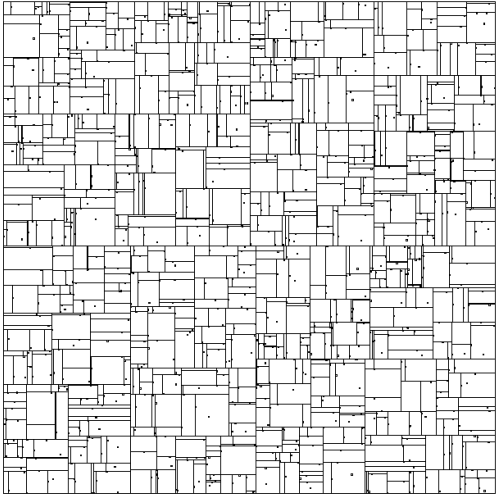
\includegraphics[scale=0.6]{./images/kd-tree.png}
\caption{Space partitioning using coordinate split \cite{Yianilos93}}
\label{fig:kd-tree}
\end{figure}
VP-trees on the other hand, uses distance from a selected vantage point as the criterion for partition. Again, the notion of distance here is arbitrary. Points near the selected point are assigned to the left child, whereas points further away are assigned to the right child.~\cite{Yianilos93} Proceeding recursively a binary tree is formed. This results in a spherical partition of space.
\begin{figure}[h]
\centering
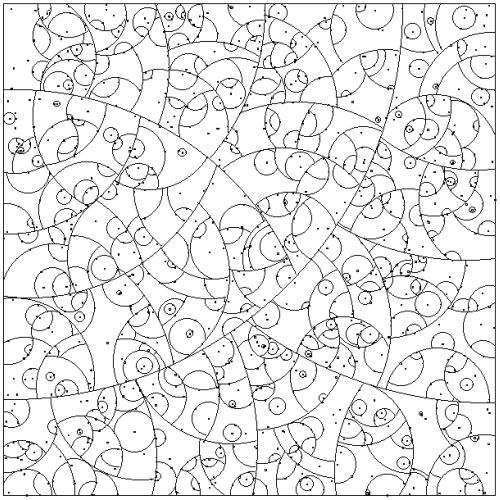
\includegraphics[scale=0.6]{./images/vp-tree.png}
\caption{Space partitioning using vantage points~\cite{Yianilos93}}
\label{fig:vp-tree}
\end{figure}
\paragraph{Conventional construction algorithm} The simplest algorithm for constructing a VP-tree follows a recursive approach. The root of the tree corresponds to the entire metric space. A function then selects, based on some pre-defined criteria, a vantage point for the root. This "distinguished" point is then used to partition the space into left and right subspaces as previously mentioned. This is repeated on the left and right child to get a binary tree. In the original algorithm outlined in~\cite{Yianilos93} the function that selects a vantage point, basis this selection on the variance in distance. The point that maximizes the variance in distance between itself and other points in the node is selected as the vantage point. 
\begin{algorithm}[h]
\caption{VP-tree construction~\cite{Yianilos93}}
\label{alg:vp-treecon}
\begin{algorithmic}[1]
\Procedure{bsttreevp}{P}
\If {$P = \phi$} \Return $\phi$
\EndIf
\State $new(node)$
\State $node.vp \gets selectvp(P)$
\State $node.center$ $\gets$ $median_{(p\ \epsilon\ P)}$ $d(vp, p)$
\State $ldata \gets \{p\ \epsilon\ P\ |\ d(vp, p) < node.center\}$
\State $rdata \gets \{p\ \epsilon\ P\ |\ d(vp, p) \geq node.center\}$
\State $node.left \gets bsttreevp(ldata)$
\State $node.right \gets bsttreevp(rdata)$
\State \Return node
\EndProcedure
\Procedure{selectvp}{P}
\State $samp \gets sample(P)$
\State $bestvar \gets 0$
\algstore{vptree}
\end{algorithmic}
\end{algorithm}

\begin{algorithm}[h]
\begin{algorithmic}[1]
\algrestore{vptree}
\For{$i\ \epsilon\ samp$}
\State $lsamp \gets sample(P)$
\State $dist \gets \{d(i, j)\ |\ j\ \epsilon\ lsamp\}$
\State $var \gets variance(dist)$
\If{$var > bestvar$} 
\State $bestvar \gets var$
\State $vp \gets i$
\EndIf
\EndFor
\State \Return $vp$
\EndProcedure
\end{algorithmic}
\end{algorithm}

\paragraph{Introducing randomness} Depending on the number points in the samples selected, the trees constructed by Algorithm 1 may or may not be deterministic. Consider the extreme case in which we evaluate all pair wise distances. In this case, we would almost always construct the same tree. For data with a large number of features and for arbitrary metric spaces, such a construction would not always yield the correct NN. Traversing to the appropriate node gives only a fraction of the NN. Despite all the effort put into constructing an optimal tree, we are limited by the constraints of dimensionality. We propose two modifications to the aforementioned VP-tree construction to make it more viable.
\begin{enumerate}
\item Truncation: Instead of subdividing the metric space continuously, we divide it until the number of points in a node falls below a threshold value. Alternatively, we impose a limit on the depth of the tree. For large data sets, this would significantly reduce the cost of construction. 
\item Randomness: We seek to introduce randomness into the process of VP-tree construction. It is known that random selection of vantage points is only slightly less optimal than the procedure described in Algorithm 1.~\cite{Yianilos93} By constructing multiple random trees, we hope to partially overcome the constraints that dimensionality puts on NN search using VP-trees. 
\end{enumerate}

\begin{algorithm}[h]
\caption{Random VP-tree construction}
\label{alg:vp-treeconr}
\begin{algorithmic}[1]
\State $MAXLVL \gets ML$
\State $MAXPNTS \gets MP$
\State $lvl \gets 0$
\Procedure{randbsttreevp}{P, lvl}
\If {$P = \phi$ or $|P| < MAXPNTS$ or $lvl > MAXLVL$}
\State $node.data \gets P$
\State \Return $node$
\EndIf
\State $new(node)$
\algstore{impvp}
\end{algorithmic}
\end{algorithm}

\begin{algorithm}[h]
\begin{algorithmic}[1]
\algrestore{impvp}
\State $node.vp \gets randselectvp(P)$
\State $node.center$ $\gets$ $median_{(p\ \epsilon\ P)}$ $d(vp, p)$
\State $ldata \gets \{p\ \epsilon\ P\ |\ d(vp, p) < node.center\}$
\State $rdata \gets \{p\ \epsilon\ P\ |\ d(vp, p) \geq node.center\}$
\State $node.left \gets randbsttreevp(ldata, lvl + 1)$
\State $node.right \gets randbsttreevp(rdata, lvl + 1)$
\State \Return node
\EndProcedure
\Procedure{randselectvp}{P}
\State $vp \gets random(P)$
\State \Return $vp$
\EndProcedure
\end{algorithmic}
\end{algorithm}

\section{Searching Random VP-Trees}
\paragraph{Psuedocode} The algorithm that we propose is based on the construction of a number of random VP-trees and searching each tree iteratively to find the NN. It is an extension of the approach mentioned in~\cite{Dasgupta15} and~\cite{Moon11}. Presented below is a brief outline of the algorithm and the psuedocode. 
\begin{enumerate}
\item Construct a random VP-tree using given points
\item Perform depth first search on the tree to get a set of NN candidates for a query.
\item Linearly search the the candidates for the best NN. 
\item If there exists a list of other NN candidates from the previous iteration, merge the lists to make a note of best NN and store them.
\item Go to step 1 and repeat until the desired accuracy is achieved. 
\end{enumerate}

\begin{algorithm}[h]
\caption{Random VP-tree search}
\label{alg:vp-treecsearch}
\begin{algorithmic}[1]
\State $MAXLVL \gets ML$
\State $MAXPNTS \gets MP$
\State $lvl \gets 0$
\State $prevnn \gets \phi$
\State $NTREE \gets NT$
\Procedure{randvpsearch}{points, query, maxnn}
\For{$i \gets 1:NTREE$}
\State $tree \gets randbsttreevp(points, lvl)$
\State $nn \gets search(tree, query, maxnn)$
\State $bestnn \gets merge(nn, prevnn)$
\State $prevnn \gets nn$
\EndFor
\algstore{impvp}
\end{algorithmic}
\end{algorithm}

\begin{algorithm}[h]
\begin{algorithmic}[1]
\algrestore{impvp}
\State \Return node
\EndProcedure
\Procedure{search}{tree, query, maxnn}
\If{$isleaf(tree)$}
\State $nn \gets linearnnsearch(tree.data, query, maxnn)$
\State \Return $nn$
\EndIf
\State $dist = d(query, tree.vp)$
\If{$dist < tree.center$}
\State \Return $search(tree.left, query, maxnn)$
\Else
\State \Return $search(tree.right, query, maxnn)$
\EndIf
\EndProcedure
\end{algorithmic}
\end{algorithm}

\paragraph{Merging} Notice the merge function defined in algorithm 3 is fairly abstract. This is because there are several different ways in which knowledge about previous NN can be incorporated into the NN search for the current iteration. We consider two separate techniques. 
\\
\emph{Problem:} Given $n$ queries $q_1,q_2,...,q_n$ and $nnmax$ neighbors $k^{i-1}_1,k^{i-1}_2,...k^{i-1}_{nnmax}$ for each query from the previous iteration, we want to find the best $nnmax$ NN for the current iteration, $k^{i}_1,k^{i}_2,...k^{i}_{nnmax}$ for each query. 
\begin{enumerate}
\item Horizontal Merge: For every iteration, we have a transient set of NN that is given by line 8 in Algorithm 3. Therefore there are two matrices:
\begin{equation}
nntrans = 
\begin{bmatrix}
nn_{1,1} & nn_{1,2} & \dots & nn_{1,nnmax} \\
nn_{2,1} & nn_{2,2} & \dots & nn_{2,nnmax} \\
\vdots   & \vdots   & \ddots & \vdots \\
nn_{n,1} & nn_{n,2} & \dots & nn_{n,nnmax}
\end{bmatrix}
k_{i-1} =
\begin{bmatrix}
k^{i-1}_{1,1} & k^{i-1}_{1,2} & \dots & k^{i-1}_{1,nnmax} \\
k^{i-1}_{2,1} & k^{i-1}_{2,2} & \dots & k^{i-1}_{2,nnmax} \\
\vdots   & \vdots   & \ddots & \vdots \\
k^{i-1}_{n,1} & k^{i-1}_{n,2} & \dots & k^{i-1}_{n,nnmax}
\end{bmatrix}
\end{equation}
For horizontal merge, we linearly search for $nnmax$ NN for each query $q_i$ by searching over the $i^{th
}$ row in $nntrans$ and $k_{i-1}$. Therefore, the optimal set of NN after iteration $i$ is given by:
\begin{equation}
k_i = 
\begin{bmatrix}
linearnnsearch([nn_{1,1},\dots, nn_{1,nnmax}, k^{i-1}_{1,1},\dots, k^{i-1}_{1,nnmax}],q_1,nnmax) \\
linearnnsearch([nn_{2,1},\dots, nn_{2,nnmax}, k^{i-1}_{2,1},\dots, k^{i-1}_{2,nnmax}],q_2,nnmax) \\
\vdots \\
linearnnsearch([nn_{n,1},\dots, nn_{n,nnmax}, k^{i-1}_{n,1},\dots, k^{i-1}_{n,nnmax}],q_n,nnmax)
\end{bmatrix}
\end{equation}
\begin{equation}
k_i = 
\begin{bmatrix}
k^{i}_{1,1} & k^{i}_{1,2} & \dots & k^{i}_{1,nnmax} \\
k^{i}_{2,1} & k^{i}_{2,2} & \dots & k^{i}_{2,nnmax} \\
\vdots   & \vdots   & \ddots & \vdots \\
k^{i}_{n,1} & k^{i}_{n,2} & \dots & k^{i}_{n,nnmax}
\end{bmatrix}
\end{equation}
This method often requires less total distance evaluations to converge to a particular accuracy valuation. However, it requires more number of iterations and correspondingly more tree constructions. It is most suited for problems for which tree construction is less expensive. 
\item Proximity Merge: In only considering the prior NN for a query $q_i$ to compute the NN for the current iteration, we are inherently losing some information present. Consider depth first search on a random VP-tree for three query points: $q_i, q_j, q_k$. Suppose the NN for all of them come from the same leaf of the tree. Then in searching for NN of $q_i$, we should not only look at prior neighbors of $q_i$, but also previous neighbors of $q_j,q_k$. We use the knowledge about proximity of different query points to optimize the search. Let $Q_i$ be the set of query points close to $q_i$. If $K_i$ is a cumulative list of all previous NN for query points in $Q_i$, $k_i$ can be computed as follows: 
\begin{equation}
k_i = 
\begin{bmatrix}
linearnnsearch([nn_{1,1},\dots, nn_{1,nnmax}, k^{i-1}_{1,1},\dots, k^{i-1}_{1,nnmax},K_1],q_1,nnmax) \\
linearnnsearch([nn_{2,1},\dots, nn_{2,nnmax}, k^{i-1}_{2,1},\dots, k^{i-1}_{2,nnmax}, K_2],q_2,nnmax) \\
\vdots \\
linearnnsearch([nn_{n,1},\dots, nn_{n,nnmax}, k^{i-1}_{n,1},\dots, k^{i-1}_{n,nnmax}, K_n],q_n,nnmax)
\end{bmatrix}
\end{equation}
\begin{equation}
k_i = 
\begin{bmatrix}
k^{i}_{1,1} & k^{i}_{1,2} & \dots & k^{i}_{1,nnmax} \\
k^{i}_{2,1} & k^{i}_{2,2} & \dots & k^{i}_{2,nnmax} \\
\vdots   & \vdots   & \ddots & \vdots \\
k^{i}_{n,1} & k^{i}_{n,2} & \dots & k^{i}_{n,nnmax}
\end{bmatrix}
\end{equation}
This algorithm is useful when tree construction is expensive. Although we end up evaluating more distances, the number of iterations taken is less. In this paper, we predominantly adopt this approach. 
\end{enumerate}

\section{Results}
\paragraph{RBF kernel} In sections 2 and 3, we have developed a general algorithm for constructing and searching random VP-trees, ignoring specifics about metric spaces. To test the method's effectiveness, we use a RBF-kernel based distance metric. Because of its ubiquitous use, the performance of the algorithm on this distance metric would be a useful parameter for measuring its success. A Gaussian radius basis function (RBF) is defined as follows~\cite{Tsuda04}:
\begin{equation}
k(x,x') = exp\ \left(\frac{||x-x'||_2^2}{2\sigma^2}\right)
\end{equation}
Using equations 1 and 2, we can transform this function so that it is a valid bounded distance metric. 
\begin{equation}
d_{RBF}(x,x') = \frac{\sqrt{2 - 2\cdot exp\left(\frac{||x-x'||_2^2}{2\sigma^2}\right)}}{1 + \sqrt{2 - 2\cdot exp\left(\frac{||x-x'||_2^2}{2\sigma^2}\right)}}
\end{equation}
This is the distance measure used for testing the algorithm on different data sets. Depending on the nature of the data set, different values for the bandwidth parameter, sigma, would have to be used so that the data spread in Hilbert space is optimal. 

\paragraph{Measures for success} We use three different parameters for evaluating how well random VP-trees behave on different data sets.
\\
\emph{Accuracy:} Given a query point $q_i$, its true NN\footnote{These are calculated by the brute force search algorithm} $k_i = \{k_1, k_2, ..., k_{nnmax}\}$, and its approximate NN $m_i = \{m_1,m_2, ..., m_{nnmax}\}$, the accuracy of the method for the single query point is given by:
\begin{equation}
acc_i = \frac{|k_i \cap m_i|}{|k_i|}
\end{equation}
The overall accuracy for $n$ query points is the average of the accuracy for all query points:
\begin{equation}
acc = \frac{1}{n}\cdot\sum\limits_{i=1}^n \left(\frac{|k_i \cap m_i|}{|k_i|}\right)
\end{equation} 
\\
\emph{Fraction of total distance evaluations:} Given $m$ database points and $n$ query points, the total number of distance evaluations calculated by the linear brute force method is $m \times n$. For the random VP-tree algorithm suppose we construct a total of $ntree$ trees and this requires $t$ distance evaluations. Additionally, assume that searching all the trees requires calculating $s$ distances. The fraction of total distance evaluations is then given by:
\begin{equation}
frac = \frac{t + s}{mn}
\end{equation}
\\
\emph{Average ratio of distance:} Given a query point $q_i$, its true NN $k_i = \{k_1, k_2, ..., k_{nnmax}\}$, and its approximate NN $m_i = \{m_1,m_2, ..., m_{nnmax}\}$, the average ratio of distance between its approximate neighbors and true neighbors is calculated as follows:
\begin{equation}
avgd_i = \frac{1}{nnmax} \cdot \sum\limits_{j = 1}^{nnmax} \left(\frac{d_{RBF}(q_i,m_{i,j})}{d_{RBF}(q,k_{i,j})}\right)
\end{equation} 
$avgd_i$ averaged over all $n$ queries gives the desired value:
\begin{equation}
avgd = \frac{1}{n} \cdot \sum\limits_{i=1}^n avgd_i
\end{equation}

\paragraph{Tests on cover type dataset} The forest cover type dataset is a geological dataset available on University of California, Irvine (UCI) Machine Learning Repository.~\cite{Blackard98}. We want to measure how NN search for RBF kernel distances compares to NN search for Euclidean distances. To make this comparison, we first sample a few points from the cover type data set. We then run a state-of-the-art kd-tree search (refer to random projection in~\cite{Moon11}) on the sample followed by the proposed random VP-tree based search. For VP-trees a RBF-kernel distance metric is used with a specified value of sigma (0.22 here). Kd-trees use the L2 norm to evaluate distance pairs. Presented below is a brief summary of the test data set and the trees used.  
\begin{center}
\begin{tabular}{l*{6}{c}r} Property & Value \\ 
\hline 
Number of points & 5,000 \\ 
Number of query points & 400 \\ 
Number of features & 54 \\ 
Number of nearest neighbors & 100 \\ 
Max. points per node & 256 \\
Tree depth & 12 \\
\end{tabular}
\captionof{table}{Running random tree search on Covtype} \label{tab:results_covtupe}
\end{center}
Both methods are iterative in nature and both find a greater percentage of NN with each iteration. Correspondingly accuracy, as defined in equation 11, would be a good measure of comparison. Following is the graph of accuracy of both the methods as a function of iteration number. 
\begin{figure}[ht]
\centering
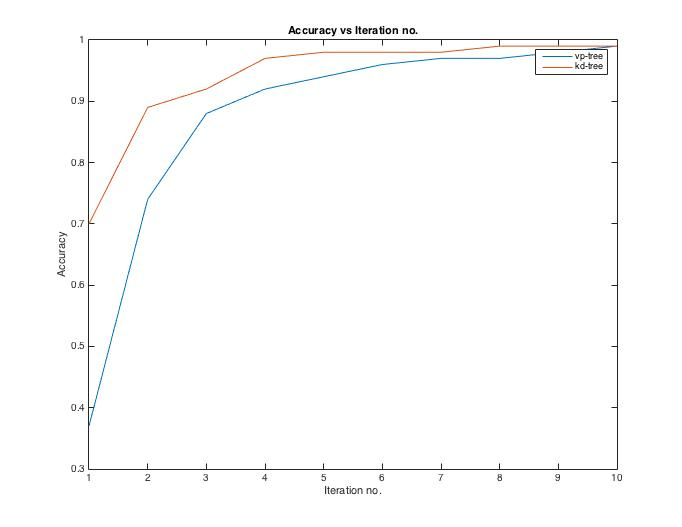
\includegraphics[scale=0.5]{./images/kdvsvp.jpg}
\caption{Accuracy vs Iteration no. for kd-trees and VP-trees}
\label{fig:vpvskd}
\end{figure}
\\
It is evident that kd-trees for Euclidean distances converge to a a larger accuracy value faster for the cover type dataset. However, VP-trees are not significantly worse. In fact, for a sufficiently large iteration no., both methods give the same accuracy value. Consider the values after 15 iterations for both the methods.
\begin{center}
\begin{tabular}{l*{6}{c}r} Property & Value \\ 
\hline 
Number of iterations & 15 \\ 
\textbf{Accuracy} & \textbf{0.997} \\
Time taken to run & 45 s \\
\end{tabular}
\captionof{table}{Running kd-tree search on Covtype} \label{tab:kd_covtupe}
\end{center}
\begin{center}
\begin{tabular}{l*{6}{c}r} Property & Value \\ 
\hline 
Number of iterations & 15 \\
RBF kernel bandwidth & 0.22 \\ 
\textbf{Accuracy} & \textbf{0.993} \\
Fraction of total distance evaluations & 2.11 \\
Average ratio of distance & 1.00 \\
Time taken to run & 1.23 s \\
\end{tabular}
\captionof{table}{Running VP-tree search on Covtype} \label{tab:vp_covtupe}
\end{center}
While the absence of a vector space is a constraint on the convergence of random VP-tree based NN search, it is not significantly worse. Runs on SUSY dataset show similar trends. 

\paragraph{Tests on SUSY dataset} SUSY is a physical data set also available on University of California, Irvine (UCI) Machine Learning Repository.~\cite{Whiteson2014} A similar set of runs as before, but using a much larger set of points helps establish the observations stated previously. Consider the following properties of the points and trees.
\begin{center}
\begin{tabular}{l*{6}{c}r} Property & Value \\ 
\hline 
Number of points & 500,000 \\ 
Number of query points & 100 \\ 
Number of features & 18 \\ 
Number of nearest neighbors & 100 \\ 
Max. points per node & 2,048 \\
Tree depth & 12 \\
\end{tabular}
\captionof{table}{Running random tree search on SUSY} \label{tab:results_susy}
\end{center}
Accuracy values for different iteration show slightly exaggerated differences in convergence rates compared to those shown in figure 3. 
\begin{figure}[ht]
\centering
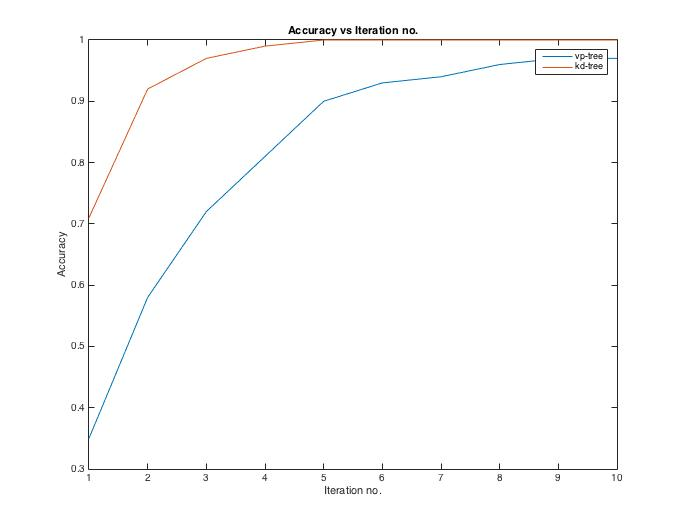
\includegraphics[scale=0.5]{./images/kdvsvpsusy.jpg}
\caption{Accuracy vs Iteration no. for kd-trees and VP-trees}
\label{fig:vpvskdsusy}
\end{figure}
\\
\pagebreak
\bibliography{reportbib}{}
\bibliographystyle{plain}

\end{document}